

\documentclass[letterpaper,11pt]{article}
\usepackage[margin=0.5in,bottom=1in,footskip=0.5in]{geometry}
%\documentclass[letterpaper,11pt]{article} %For use in US
\usepackage{latexsym}
\usepackage[empty]{fullpage}
\usepackage{titlesec}
\usepackage{marvosym}
\usepackage[usenames,dvipsnames]{color}
\usepackage{verbatim}
\usepackage{enumitem}
\usepackage[hidelinks]{hyperref}
\usepackage[english]{babel}
\usepackage{tabularx}
\usepackage{tikz}
\usepackage{graphicx}
\input{glyphtounicode}


% serif
 \usepackage{palatino}
% \usepackage{times} %This is the default as well
% \usepackage{charter}

% sans-serif
% \usepackage{helvet}
% \usepackage[sfdefault]{noto-sans}
% \usepackage[default]{sourcesanspro}

%-----PAGE SETUP---------------------------------------------------------------


% Margins for US Letter size
\addtolength{\oddsidemargin}{-0.5in}
\addtolength{\evensidemargin}{-0.5in}
\addtolength{\textwidth}{1in}
\addtolength{\topmargin}{-.5in}
\addtolength{\textheight}{1.0in}

\urlstyle{same}

\raggedbottom
\raggedright
\setlength{\tabcolsep}{0cm}

% Sections formatting
\titleformat{\section}{
  \vspace{-4pt}\scshape\raggedright\large
}{}{0em}{}[\color{black}\titlerule \vspace{-5pt}]

% Ensure that .pdf is machine readable/ATS parsable
\pdfgentounicode=1

%-----CUSTOM COMMANDS FOR FORMATTING SECTIONS----------------------------------
\newcommand{\CVItem}[1]{
  \item\small{
    {#1 \vspace{-2pt}}
  }
}

\newcommand{\CVSubheading}[4]{
  \vspace{-2pt}\item
    \begin{tabular*}{0.97\textwidth}[t]{l@{\extracolsep{\fill}}r}
      \textbf{#1} & #2 \\
      \small#3 & \small #4 \\
    \end{tabular*}\vspace{-7pt}
}

\newcommand{\CVSubSubheading}[2]{
    \item
    \begin{tabular*}{0.97\textwidth}{l@{\extracolsep{\fill}}r}
      \text{\small#1} & \text{\small #2} \\
    \end{tabular*}\vspace{-7pt}
}

\newcommand{\CVSubItem}[1]{\CVItem{#1}\vspace{-4pt}}

\renewcommand\labelitemii{$\vcenter{\hbox{\tiny$\bullet$}}$}

\newcommand{\CVSubHeadingListStart}{\begin{itemize}[leftmargin=0.5cm, label={}]}
% \newcommand{\resumeSubHeadingListStart}{\begin{itemize}[leftmargin=0.15in, label={}]} % Uncomment for US
\newcommand{\CVSubHeadingListEnd}{\end{itemize}}
\newcommand{\CVItemListStart}{\begin{itemize}}
\newcommand{\CVItemListEnd}{\end{itemize}\vspace{-5pt}}

%------------------------------------------------------------------------------
% CV STARTS HERE  %
%------------------------------------------------------------------------------
\begin{document}

%-----TITLE----------------------------------------------------------------

\begin{minipage}[c]{0.2\textwidth}
    \begin{tikzpicture}
        % Adjust the positioning of the image to the left
        \node at (-0.5,0) {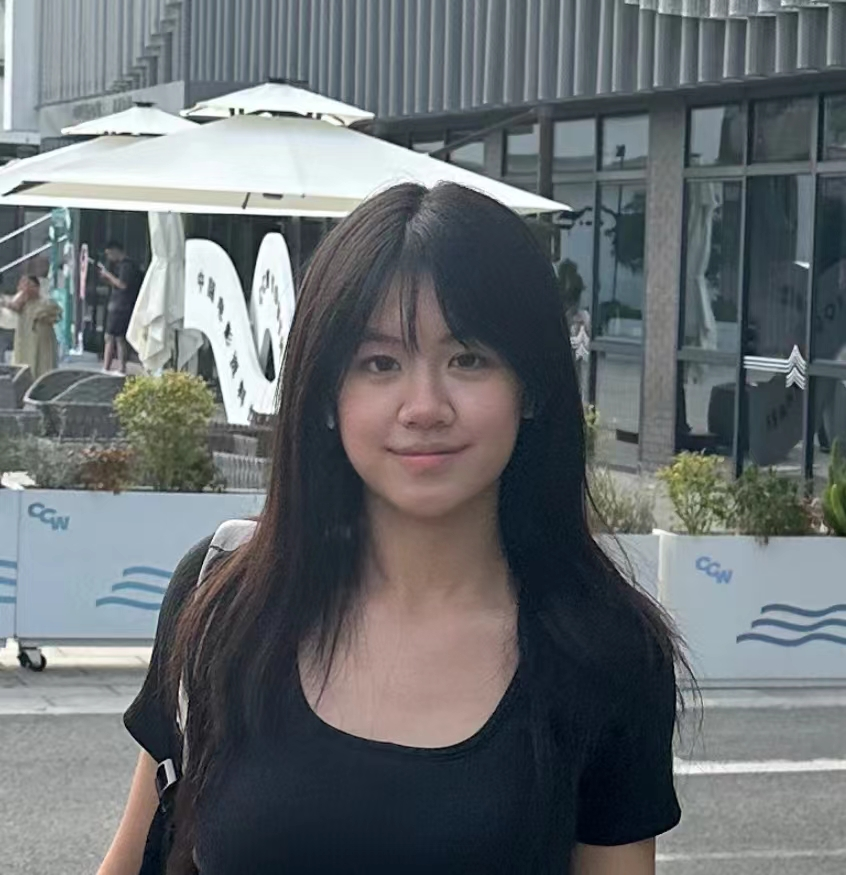
\includegraphics[width = 4cm]{portrait.jpg}}; 
        % Adjust 'width' and 'at' coordinates to fit the image and layout
    \end{tikzpicture}
\end{minipage}
\begin{minipage}[c]{0.05\textwidth}
\-\
\end{minipage}
\begin{minipage}[c]{0.5\textwidth}
    \textbf{\Huge \scshape{Sandy (Yuelin) Hou}} \\ \vspace{1pt} 
    % \scshape sets small capital letters, remove if desired
    \small{+86 18971178310} \\
    \href{yh405@duke.edu}{\underline{yh405@duke.edu}}\\
    \href{https://github.com/Sandyuelin}{\underline{Github @Sandy Hou}}
\end{minipage}


%-----EDUCATION----------------------------------------------------------------
\section{Education}
  \CVSubHeadingListStart
%    \CVSubheading % Example
%      {Degree Achieved}{Years of Study}
%      {Institution of Study}{Where it is located}
    \CVSubheading
      {{Duke Kunshan University (DKU) $ | $ \emph{\small{Computer Science}}}}{Aug. 2023 -- Present}
      {- GPA: 3.7 \\
      - Dean's List,Fall 2023 \\ 
      - Chancellor’s Scholarship \& UGRD Entrance Scholarship} {Kunshan, China}
    \CVSubheading
      {{Wuhan No.2 High School}}{Aug. 2020 -- Jun. 2023}
      {- College Entrance Exam (Science-track) - Top 8000/150,000+}{Wuhan, China}
  \CVSubHeadingListEnd


%-----Research Experience----------------------------------------------------------------

\section{Research Experience}
  \CVSubHeadingListStart
%    \CVSubheading %Example
%      {What you did}{When you worked there}
%      {Who you worked for}{Where they are located}
%      \CVItemListStart
%        \CVItem{Why it is important to this employer}
%      \CVItemListEnd
    \CVSubheading
      {Chinese Calligraphy Recognition}{Jun. 2024 -- Sept. 2024}
      {Wangxuan Computer Science Institute of Peking University}{Beijing, China}
      \CVItemListStart
        \CVItem{Worked on Chinese character classifier to distinguish simplified and complex version}
        \CVItemListStart
        \CVItem{Preprocess image and create calligraphy using PIL}
        \CVItem{Extract the latents of both created data and existing data}
        \CVItem{Classify the character by calculating the cosine similarity of latents}
      \CVItemListEnd
        \CVItem{Utilize labelme to process 2500+ image data}
        \CVItem{Self-learning computer vision related materials and papers}
      \CVItemListEnd
  \CVSubHeadingListEnd





%-----Project----------------------------------------------------------------

\section{Side Projects}
  \CVSubHeadingListStart
%    \CVSubheading
%      {Title of Work}{When it was done}
%      {Institution you worked with}{unused}
    \CVSubheading
      {{Impact Benchmarking Analysis on Electric Vehicle’s Sustainability} }{Sept. 2023 -- Nov. 2023}
      {DKU University-Corporation Innovation Lab (U-Corp)}{Kunshan, China}
       \CVItemListStart
        \CVItem{Co-authored an analysis on the sustainability of EV battery recycling as \href{https://ine.dukekunshan.edu.cn/project/23f-u-corp-impact-bread/#1709088351127-4a381d9f-3e83}{\underline{U-Corp Final Report}}}
        \CVItem{Conducted comparative analysis on battery recycling between industry leaders and new startups }
    \CVItemListEnd
    
  \CVSubHeadingListEnd

%-----CONFERENCES AND PRESENTATIONS--------------------------------------------
\iffalse
\begin{comment}
Again the title should have already been enough, but if it is necessary to add
descriptions maintain the consistency from prior sections
\end{comment}

\section{Conferences and Presentations}
  \CVSubHeadingListStart
%    \CVSubheading % Example
%      {Work Presented}{When}
%      {Occasion}{}
    \CVSubheading
      {Photometric Filter Fidelity and Use for Be Star Identification}{November 2017}
      {Austin College Physics Research Seminar}{}
    \CVSubheading
      {Reflectometry for Volumetric Soil Moisture Measurement}{May 2017}
      {Austin College Atmospheric Physics Fair}{}
    \CVSubheading
      {Design and Manufacturing of Products using 3D Printing}{April 2017}
      {Austin College Student Scholarship Conference}{}
  \CVSubHeadingListEnd

%-----HONORS AND AWARDS--------------------------------------------------------
\section{Honors and Awards}
  \CVSubHeadingListStart
%    \CVSubheading %Example
%      {What}{When}
%      {Short Description}{}
    \CVSubheading
      {Dean's List}{Fall 2017}
      {Recognition for to 20\% of students in academics at Austin College}{}
    \CVSubheading
      {Noyce STEM Education Leadership Scholarship}{June 2017}
      {Merit based grant for students pursuing education in STEM fields}{}
    \CVSubheading
      {Stephens Scholarship}{May 2017}
      {Merit based scholarship to support international study experiences within Austin College}{}
    \CVSubheading
      {John D . Mosely Scholarship}{July 2016}
      {Merit based scholarship requiring Austin College alumnus nomination}{}
    \CVSubheading
      {Presidents List}{Spring 2016}
      {Overall GPA above 3.8 at Austin College}{}
    \CVSubheading
      {Eagle Scout}{April 2006}
      {Highest level of achievement within the Boy Scouts of America}{}
  \CVSubHeadingListEnd

%-----TEACHING EXPERIENCE------------------------------------------------------
\begin{comment}
Section is here as it applied to my application for positions in academia. 
Remember to tailor the resume for to the position.
\end{comment}

\section{Teaching Experience}
  \CVSubHeadingListStart
%    \CVSubheading
%      {What}{When}
%      {School}{Where}
    \CVSubheading
      {High School Physics (11 Weeks Teaching/Observing)}{Fall 2017}
      {Denison High School}{Denison, TX}
    \CVSubheading
      {High School Calculus (11 Weeks Teaching/Observing)}{Fall 2017}
      {Denison High School}{Denison, TX}
    \CVSubheading
      {High School Geometry (9 Weeks Teaching/Observing)}{Spring 2016}
      {Sherman High School}{Sherman, TX}
  \CVSubHeadingListEnd
\fi


%-----COMMUNITY INVOLVEMENT----------------------------------------------------
\section{Community Involvement}
  \CVSubHeadingListStart
    \CVSubheading
      {Senior Associate in DKU Sports Complex}{Aug. 2023 -- Present}
      {- Coordinated staff and managed equipment, ensuring smooth daily operations.\\
         - Enforced safety protocols to maintain a secure environment for 1w + members.}{}
    \CVSubheading
      {Treasurer of DKU Running Club(DKURC)}{Nov. 2023 -- Present}
      {- Oversaw club finances, managing the budget and tracking expenses.\\
         - Assisted in overall event coordination \& club practice \& administration for \href{https://sites.duke.edu/dkurunning/leadership/}{\underline{DKURC}}\\
         - Handled reimbursements for 8 events and managed merchandise worth 3000 RMB.}{}
    \CVSubheading
      {Interviewer \& Writer of DKU Club TT101 (Talking to 101 Professors)}{Sept. 2023 -- Present}
      {- Conducted 1v1 and 3v1 interviews with 5 DKU professors\\
        - Authored bilingual articles in Chinese and English to club's WeChat Official Account.}{}
        \CVItem{- Highlighted works include:}
          \begin{itemize}[left=2em, itemsep=2pt, parsep=2pt]
            \CVItem{\href{https://mp.weixin.qq.com/s/LriD9cSZHalxBJbugd_jXQ}{\underline{Interview with Professor Pascal Grange: Merging the Beauty of Science and Art}}}
            \CVItem{\href{https://mp.weixin.qq.com/s/ZeKLnIZEenoQfteYwf-mSw}{\underline{Interview with Professor Kevin Sprague: A Winding Path Lies Ahead, Yet Progress Shall Lead Us There}}}
            
          \end{itemize}
  \CVSubHeadingListEnd


%-----SKILLS-------------------------------------------------------------------
\begin{comment}
This section is compressed from the various skills sections that Euro CV
recommends.
\end{comment}

\section{Skills}
 \begin{itemize}[leftmargin=0.5cm, label={}]
    \small{\item{
     \textbf{Natural Languages}{: English (Fluent), Chinese(Native), Swedish(Beginner-level)} \\
     \textbf{Programming Languages}{: Python (NumPy, PyTorch, SciPy, Matplotlib, Pandas), Java, LaTex} \\
     \textbf{Certificates}{: TOFEL(102), IELTS(7.0), CPR(cardiopulmonary resuscitation training)} \\
     \textbf{Hobbies}{: Running(competed 10km run \& 12km cross-country run in Suzhou), Frisbee(affiliated to DKU Ultimate Frisbee Varsity team), Climbing (hosted DKU Climbing Wall Orientation Video)} \\
    }}
 \end{itemize}
    
%------------------------------------------------------------------------------
\end{document}